% chapter 5
\cleardoublepage
\phantomsection
\chapter{Results and Discussion}
My final chapter, Results and Discussion, aims to offer a comprehensive overview of my system's performance through the acquisition and analysis of results. To acquire these results, I plan on taking a sample of seven results from the system with all five available, followed by a further seven results using only four nodes and so on until there is only one node online.

The values for each cycle will then be averaged and a graph presented. A discussion on this graph will offer insight into the behaviour of my system; my hypothesis being that an increase in performance will be rapid at first but will ultimately be tempered by granularity as resources begin to become scarcer.

After I have discussed the results of my system's performance, I will finalise this chapter by touching on improvements that could be made to my system as well as aspects I believe went well in hindsight.

\section{Acquisition and analysis of results: Cluster performance measured by time taken}
The first stage in my discussion on results is acquisition. In order to collect results with a good degree of provenance, I need to mitigate or remove any environment variables that could cause a drastic change in the system's computing capacity during my code execution.

To this end, I have mitigated for instability by shutting down non-essential machines running on the hypervisor and have run all of my tests during the night-time when load should be much lower. I have also halted my web server's MySQL database and disabled PHP processing so no server pre-processing occurs there. This will, to the best of my ability, remove any Internet load that might affect the server.

\textbf{\sffamily{Collecting and presenting results: Continued effort creep issues}}

The results-collecting process took approximately two hours, excluding the momentary pauses that happened while I modified the configuration files between batch runs. The entire, unedited console outputs can be found in Appendix γ, however for convenience I will now list the averages from each configuration.

\begin{itemize}
    \item \textbf{One node} took approx. 426 417 ms to complete approx. 1 048 630 000 000 000 program loops.
    \item \textbf{Two nodes} took approx. 219 426 ms to complete approx. 1 048 670 000 000 000 program loops.
    \item \textbf{Three nodes} took approx. 145 995 ms to complete approx. 1 048 690 000 000 000 program loops.
    \item \textbf{Four nodes} took approx. 110 373 ms to complete approx. 1 048 730 000 000 000 program loops.
    \item \textbf{Five nodes} took approx. 87 939 ms to complete approx. 1 048 770 000 000 000 program loops.
\end{itemize}

Initial presentation of my results shows promise, with a clear downward trend in the amount of time the search takes place based on the number of nodes online in the system. One might also be able to identify the effects of granularity on my system simply by identifying the closing gap between the average times from each set of runs.

As I have already discussed in detail in Chapter 4, my system is still experiencing effort creep not appearing to be in any logical increments between batch runs but always the same within batches. The creep is typically somewhere in the range of 40 billion loops, give or take, between groups. To calculate how much drift each run may be experiencing, I can work out how much as a percentage the difference between each batch has compared to my single-node system.

\begin{itemize}
    \item \textbf{One node} is our benchmark, with approx. 1 048 630 000 000 000 program loops
    \item \textbf{Two nodes} have crept up by 40 000 000 000 loops from my single-node batch (0,00381\% increase)
    \item \textbf{Three nodes} have crept up by 60 000 000 000 loops from my single-node batch (0,00572\% increase)
    \item \textbf{Four nodes} have crept up by 100 000 000 000 loops from my single-node batch (0,00954\% increase)
    \item \textbf{Five nodes} have crept up by 140 000 000 000 loops from my single-node batch (0,01335\% increase)
\end{itemize}

As one can see, the overall increase in effort, while sub-optimal, does not skew my results by results by more than 0,01\% in total. I personally feel that these sorts of values do not pose a substantial threat to my research sufficiently enough to require a revisit of Chapter 4. Indeed, the worst-case scenario changes the results from the five-node cluster by an average of only 11 ms.

\textbf{\sffamily{Collecting and presenting results: Insight using network statistics}}

Another metric that may be useful in measuring a Beowulf cluster's performance is its network footprint. This might be its bandwidth usage or the latency between nodes (as posited by Shipman et. al. \cite{shipman_et_al_2006}). This method of measuring a cluster's performance is typical when comparing two cluster APIs but doesn't appear to be common when ascertaining a cluster's computational power.

That in mind, using network metrics can also be informative when measuring granularity. Typically in a standard Beowulf cluster, it is the network which offers the greatest possibility of system bottle-necking. The cluster I have developed does not use standard networking largely due to its virtualised nature. This makes measuring network bottle-necking unnecessary and pointless, as any bottle-neck is going to be inside the CPU or between buses rather than inside the virtual network.

\textbf{\sffamily{Collecting and presenting results: A visual representation}}

Returning at last to the discussion on my results, in order to get a better visual idea of what is happening with the timed results, I will now present my data on a line chart. I expect to see a rapid decrease in the time taken to execute my software followed by a plateauing of the speedup, in line with the first list in this section.

\begin{figure}[H]
    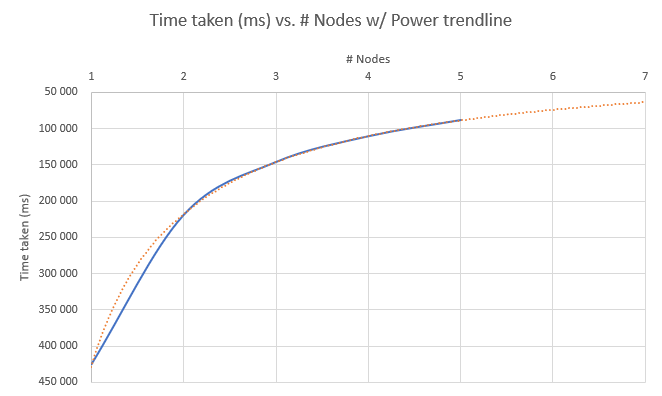
\includegraphics[width=\linewidth]{CITY3111/bitmaps/figure_21.png}
    \caption{Line chart demonstrating predicted granularity occurring in my cluster}
    \label{figure_21}
\end{figure}

As suspected, my initial data-points when mapped on a smoothed line graph suggest a clear downward trend in time taken to perform full execution followed by a plateauing. Using a crude trend algorithm of $y = a \times x^{b}$ to predict a future trend, it can reasonably be posited that in this cluster's case with this particular problem or implementation, more than five nodes would not return a significant enough decrease in execution time to justify its resource usage or time to maintain.

The system I have created demonstrates that simply by combining the computational effort of several interconnected machines of unremarkable quality, a speedup close to the number of additional nodes is possible up to approximately five nodes. In better circumstances, I would acquire dedicated hardware for each node and improve my software further and expect a better speedup across more nodes.

\section{Brief discussion on project: Comments on project completion \& future work}
With the conclusion of my project, it is now appropriate for me to retrospectively discuss the events that lead us to this point. Specifically, I intend on discussing points of merit, failings and potential future iterations on this concept.

\textbf{\sffamily{Views on project \& results}}

HPC is a field of computing that has existed for some time now, indeed nothing in this dissertation can be regarded as novel. That is not the purpose of my writings. What is, however, is my personal knowledge gain and to that end I feel appropriately satisfied with the progress I have made in understanding how Beowulf clusters are constructed, maintained and programmed for.

In my view, the project was largely a success, with my cluster performing well under varying workloads utilising the custom software I designed to run atop the MPI runtime. Improvements can always be made, both in hardware and software, regardless of the complexity of the system or its problem.

For example, utilising a dedicated server rather than independent hardware for each node is sub-optimal for a number of reasons that have been covered in prior chapters, and my software has some clear bugs that would need to be addressed before it could be considered a production tool. However, in the bigger picture presented, these issues are not of detriment to the project's goals.

\textbf{\sffamily{Future work}}

This project has a wide scope for future research. I've explored the MPI paradigm as a method of inter-nodal computation in this project, however APIs like GASnet \cite{gasnet_team_2020} offer a lower-level alternative to what is viewed by some a limiting tool-set.

Possibly using different APIs with more cutting-edge problems would be an area of research I would have a great degree of interest in pursuing. As computer science moves into a world of increasing problem sizes, supercomputer systems are going to be required more than ever to assist in research across an ever-broadening range of subjects. My hope is that this project can become a staging piece for my continued work within this field of academia in due course.
